% REV-ECIT 2026 — Tiểu ban AI và ứng dụng liên ngành. Bản v2 (bản nộp).
% Bản v1 (bài phương pháp, đủ TN1 + TN2 + panel) nằm ở ../rev-ecit2026/, tag git
% rev-ecit2026-v1, và là seed cho bài tạp chí. Bản này là bài ỨNG DỤNG: mô hình tổng quát,
% một bảng kết quả benchmark, một trường hợp minh họa qua web app; không nêu tên hệ.
% Quy cách: tiếng Việt, IEEE conference, A4, tối đa 6 trang.
% Biên dịch: ./compile.sh (XeLaTeX). Số liệu: make_tables.py -> generated/ (bảng benchmark
% từ pooled_comparison.json; số liệu trường hợp triển khai từ case/run/, bản sao run của web app).
\documentclass[conference,a4paper]{IEEEtran}

\usepackage{fontspec}
\setmainfont{texgyretermes}[
  Extension=.otf,
  UprightFont=*-regular, BoldFont=*-bold,
  ItalicFont=*-italic, BoldItalicFont=*-bolditalic]
\usepackage{cite}
\usepackage{amsmath,amssymb}
\usepackage{graphicx}
\usepackage{booktabs}
\usepackage{array}
\usepackage{url}
% Liên kết bấm được cho \cite, \ref và URL; hidelinks bỏ khung màu (quy ước của hội nghị).
\usepackage[hidelinks]{hyperref}

\graphicspath{{figures/}}
% Generated by make_tables.py — do not edit.
\newcommand{\NScen}{30}
\newcommand{\cmpAGAddie}{59.0}
\newcommand{\cmpAGAddieSD}{2.8}
\newcommand{\cmpAGTraj}{69.7}
\newcommand{\cmpAGTrajSD}{5.9}
\newcommand{\cmpAGTotal}{62.2}
\newcommand{\cmpAGTotalSD}{2.3}
\newcommand{\cmpAGMin}{86}
\newcommand{\cmpAGTok}{282}
\newcommand{\cmpAGCalls}{70}
\newcommand{\cmpEduAddie}{30.0}
\newcommand{\cmpEduAddieSD}{19.8}
\newcommand{\cmpEduAddieDiff}{28.9}
\newcommand{\cmpEduAddieP}{${<}\,0.001$}
\newcommand{\cmpEduAddieCILo}{22.3}
\newcommand{\cmpEduAddieCIHi}{36.5}
\newcommand{\cmpEduTraj}{53.0}
\newcommand{\cmpEduTrajSD}{32.7}
\newcommand{\cmpEduTrajDiff}{16.6}
\newcommand{\cmpEduTrajP}{${=}\,0.889$}
\newcommand{\cmpEduTrajCILo}{5.8}
\newcommand{\cmpEduTrajCIHi}{30.5}
\newcommand{\cmpEduTotal}{36.9}
\newcommand{\cmpEduTotalSD}{23.2}
\newcommand{\cmpEduTotalDiff}{25.3}
\newcommand{\cmpEduTotalP}{${<}\,0.001$}
\newcommand{\cmpEduTotalCILo}{17.5}
\newcommand{\cmpEduTotalCIHi}{34.5}
\newcommand{\cmpEduMin}{14}
\newcommand{\cmpEduTok}{70}
\newcommand{\cmpEduCalls}{16}
\newcommand{\cmpBaseAddie}{43.4}
\newcommand{\cmpBaseAddieSD}{17.7}
\newcommand{\cmpBaseAddieDiff}{15.6}
\newcommand{\cmpBaseAddieP}{${<}\,0.001$}
\newcommand{\cmpBaseAddieCILo}{9.9}
\newcommand{\cmpBaseAddieCIHi}{22.1}
\newcommand{\cmpBaseTraj}{69.2}
\newcommand{\cmpBaseTrajSD}{19.0}
\newcommand{\cmpBaseTrajDiff}{0.4}
\newcommand{\cmpBaseTrajP}{${=}\,0.147$}
\newcommand{\cmpBaseTrajCILo}{-4.4}
\newcommand{\cmpBaseTrajCIHi}{10.5}
\newcommand{\cmpBaseTotal}{51.1}
\newcommand{\cmpBaseTotalSD}{16.6}
\newcommand{\cmpBaseTotalDiff}{11.0}
\newcommand{\cmpBaseTotalP}{${<}\,0.001$}
\newcommand{\cmpBaseTotalCILo}{6.5}
\newcommand{\cmpBaseTotalCIHi}{18.3}
\newcommand{\cmpBaseMin}{3}
\newcommand{\cmpBaseTok}{10}
\newcommand{\cmpBaseCalls}{1}
\newcommand{\cmpReactAddie}{59.1}
\newcommand{\cmpReactAddieSD}{6.7}
\newcommand{\cmpReactAddieDiff}{-0.1}
\newcommand{\cmpReactAddieP}{${=}\,0.730$}
\newcommand{\cmpReactAddieCILo}{-2.3}
\newcommand{\cmpReactAddieCIHi}{2.0}
\newcommand{\cmpReactTraj}{71.5}
\newcommand{\cmpReactTrajSD}{9.5}
\newcommand{\cmpReactTrajDiff}{-1.9}
\newcommand{\cmpReactTrajP}{${=}\,0.633$}
\newcommand{\cmpReactTrajCILo}{-5.8}
\newcommand{\cmpReactTrajCIHi}{3.0}
\newcommand{\cmpReactTotal}{62.8}
\newcommand{\cmpReactTotalSD}{4.9}
\newcommand{\cmpReactTotalDiff}{-0.6}
\newcommand{\cmpReactTotalP}{${=}\,1.000$}
\newcommand{\cmpReactTotalCILo}{-2.6}
\newcommand{\cmpReactTotalCIHi}{1.1}
\newcommand{\cmpReactMin}{5}
\newcommand{\cmpReactTok}{15}
\newcommand{\cmpReactCalls}{5}
\newcommand{\cmpAddieAddie}{48.5}
\newcommand{\cmpAddieAddieSD}{3.6}
\newcommand{\cmpAddieAddieDiff}{10.5}
\newcommand{\cmpAddieAddieP}{${<}\,0.001$}
\newcommand{\cmpAddieAddieCILo}{9.2}
\newcommand{\cmpAddieAddieCIHi}{11.9}
\newcommand{\cmpAddieTraj}{81.5}
\newcommand{\cmpAddieTrajSD}{3.0}
\newcommand{\cmpAddieTrajDiff}{-11.8}
\newcommand{\cmpAddieTrajP}{${<}\,0.001$}
\newcommand{\cmpAddieTrajCILo}{-14.0}
\newcommand{\cmpAddieTrajCIHi}{-9.7}
\newcommand{\cmpAddieTotal}{58.4}
\newcommand{\cmpAddieTotalSD}{2.7}
\newcommand{\cmpAddieTotalDiff}{3.8}
\newcommand{\cmpAddieTotalP}{${<}\,0.001$}
\newcommand{\cmpAddieTotalCILo}{2.5}
\newcommand{\cmpAddieTotalCIHi}{5.0}
\newcommand{\cmpAddieMin}{7}
\newcommand{\cmpAddieTok}{23}
\newcommand{\cmpAddieCalls}{14}
\newcommand{\cmpDickAddie}{58.0}
\newcommand{\cmpDickAddieSD}{3.0}
\newcommand{\cmpDickAddieDiff}{1.0}
\newcommand{\cmpDickAddieP}{${=}\,0.532$}
\newcommand{\cmpDickAddieCILo}{-0.5}
\newcommand{\cmpDickAddieCIHi}{2.4}
\newcommand{\cmpDickTraj}{72.6}
\newcommand{\cmpDickTrajSD}{5.6}
\newcommand{\cmpDickTrajDiff}{-3.0}
\newcommand{\cmpDickTrajP}{${=}\,0.222$}
\newcommand{\cmpDickTrajCILo}{-5.9}
\newcommand{\cmpDickTrajCIHi}{0.2}
\newcommand{\cmpDickTotal}{62.4}
\newcommand{\cmpDickTotalSD}{3.1}
\newcommand{\cmpDickTotalDiff}{-0.2}
\newcommand{\cmpDickTotalP}{${=}\,1.000$}
\newcommand{\cmpDickTotalCILo}{-1.5}
\newcommand{\cmpDickTotalCIHi}{1.2}
\newcommand{\cmpDickMin}{7}
\newcommand{\cmpDickTok}{26}
\newcommand{\cmpDickCalls}{10}
\newcommand{\cmpRpisdAddie}{58.4}
\newcommand{\cmpRpisdAddieSD}{2.5}
\newcommand{\cmpRpisdAddieDiff}{0.6}
\newcommand{\cmpRpisdAddieP}{${=}\,0.532$}
\newcommand{\cmpRpisdAddieCILo}{-0.8}
\newcommand{\cmpRpisdAddieCIHi}{1.8}
\newcommand{\cmpRpisdTraj}{69.9}
\newcommand{\cmpRpisdTrajSD}{3.3}
\newcommand{\cmpRpisdTrajDiff}{-0.2}
\newcommand{\cmpRpisdTrajP}{${=}\,0.972$}
\newcommand{\cmpRpisdTrajCILo}{-2.7}
\newcommand{\cmpRpisdTrajCIHi}{1.9}
\newcommand{\cmpRpisdTotal}{61.8}
\newcommand{\cmpRpisdTotalSD}{1.9}
\newcommand{\cmpRpisdTotalDiff}{0.4}
\newcommand{\cmpRpisdTotalP}{${=}\,1.000$}
\newcommand{\cmpRpisdTotalCILo}{-0.7}
\newcommand{\cmpRpisdTotalCIHi}{1.4}
\newcommand{\cmpRpisdMin}{10}
\newcommand{\cmpRpisdTok}{61}
\newcommand{\cmpRpisdCalls}{21}
\newcommand{\cmpMaxPAddieBetter}{${<}\,0.001$}
\newcommand{\cmpMaxPTrajBetter}{--}
\newcommand{\cmpMaxPTotalBetter}{${<}\,0.001$}
\newcommand{\cmpTokRatioReact}{18}
\newcommand{\JudgeSD}{8.7}
\newcommand{\caseObj}{5}
\newcommand{\caseMod}{3}
\newcommand{\caseTask}{3}
\newcommand{\caseAct}{10}
\newcommand{\caseMat}{3}
\newcommand{\caseSess}{8}
\newcommand{\caseItem}{8}
\newcommand{\caseCovTwo}{100}
\newcommand{\caseCovThree}{100}
\newcommand{\caseCovFour}{100}
\newcommand{\caseClosed}{5}
\newcommand{\caseViol}{8}
\newcommand{\caseViolAgent}{2}
\newcommand{\caseViolHarness}{0}
\newcommand{\caseViolOpen}{6}
\newcommand{\caseOverrunMods}{2}
\newcommand{\caseMediaMismatch}{2}
\newcommand{\caseDesign}{35}
\newcommand{\caseLocalRewrite}{4}
\newcommand{\caseLocalCheck}{8}
\newcommand{\caseLocalOutside}{23}
\newcommand{\caseLocalObjective}{ILO-03}
\newcommand{\caseMatSessions}{3}
\newcommand{\caseActMinutes}{45}
\newcommand{\caseTaskObjs}{2}
\newcommand{\caseTaskActs}{4}
\newcommand{\caseDiagOnly}{2}
\newcommand{\caseDiagOnlyIds}{ILO-01 và ILO-02}
\newcommand{\caseDiagWeight}{0}
\newcommand{\caseWeight}{20}
\newcommand{\caseMin}{10}
\newcommand{\caseTok}{301}
\newcommand{\caseCalls}{55}

\renewcommand{\figurename}{Hình}
\renewcommand{\tablename}{Bảng}
\renewcommand{\refname}{TÀI LIỆU THAM KHẢO}
\renewcommand{\abstractname}{Tóm tắt}
\renewcommand{\IEEEkeywordsname}{Từ khóa}

\begin{document}

\title{Ứng dụng hệ đa tác tử dựa trên\\
mô hình ngôn ngữ nhỏ trong thiết kế giảng dạy}

\author{\IEEEauthorblockN{Bùi Việt Phương\textsuperscript{1}, Bùi Văn Tâm\textsuperscript{2}, Phạm Văn Hải\textsuperscript{1,*}}
\IEEEauthorblockA{\textsuperscript{1}Trường Công nghệ Thông tin và Truyền thông, Đại học Bách khoa Hà Nội\\
\textsuperscript{2}Khoa Công nghệ Thông tin, Trường Đại học Hải Phòng\\
Email: phuong.bv242011m@sis.hust.edu.vn, tambv@dhhp.edu.vn, haipv@soict.hust.edu.vn\\
\textsuperscript{*}Tác giả liên hệ}}

\maketitle

\begin{abstract}
Các hệ tác tử dựa trên mô hình ngôn ngữ lớn (LLM) cho thiết kế giảng dạy (ISD) phần lớn dựa
vào LLM thương mại gọi qua API, trong khi các cơ sở giáo dục có nhu cầu dùng mô hình ngôn ngữ nhỏ
(SLM) vận hành tại chỗ. Với SLM, sự căn chỉnh giữa mục tiêu, hoạt động và đánh giá có thể bị
phá vỡ mà khó được phát hiện. Bài báo đề xuất một hệ đa tác tử thiết kế giảng dạy, trong đó các tác
tử theo vai thực hiện sáu công đoạn và dùng chung một đồ thị căn chỉnh. Khung điều phối ghi và
kiểm tra các quan hệ căn chỉnh, rồi xuất đồ thị cùng sổ vi phạm để giảng viên truy vết; đồ thị
này cũng cho phép mở rộng sang cải tiến cục bộ. Hệ được đóng gói thành ứng dụng web và được
minh họa qua việc thiết kế một học phần. Trên \NScen{} kịch bản của
ISD-Agent-Bench với Qwen3.5-2B, điểm ADDIE của hệ (\cmpAGAddie) không khác biệt có ý nghĩa thống kê với
tác tử mạnh nhất của benchmark là React-ADDIE (\cmpReactAddie).
\end{abstract}

\begin{IEEEkeywords}
hệ đa tác tử (multi-agent system); mô hình ngôn ngữ nhỏ (small language model);
thiết kế giảng dạy (instructional design); căn chỉnh kiến tạo (constructive
alignment); học liệu số (digital learning materials)
\end{IEEEkeywords}

\section{GIỚI THIỆU}
\label{sec:intro}

Thiết kế giảng dạy (Instructional Systems Design -- ISD) là quá trình xây dựng một khóa học,
từ phân tích nhu cầu đến kế hoạch triển khai. Mô hình ADDIE tổ chức quá trình này thành năm
pha: phân tích, thiết kế, phát triển, triển khai và đánh giá~\cite{branch2009addie}. Với giảng
viên, mỗi pha đòi hỏi nhiều công sức: viết mục tiêu, ra đề, thiết kế hoạt động, soạn học liệu và
lập kế hoạch từng buổi. Các hệ tác tử dựa trên mô hình ngôn ngữ lớn (Large Language Model --
LLM) đã có thể tự động hóa nhiều phần của quy trình này, từ kế hoạch bài giảng đến trọn bộ
học liệu của một khóa học~\cite{zeng2026coma,zhang2025eduplanner,yao2025instructionalagents}.
Bộ đánh giá chuẩn (benchmark) ISD-Agent-Bench so sánh các tác tử ISD trên một tập kịch bản
chung~\cite{isdagentbench}.

Tuy nhiên, các hệ tác tử ISD nói trên chủ yếu được xây dựng và kiểm chứng trên LLM cỡ lớn, phần
lớn là LLM thương mại gọi qua API. Chi phí và nguồn lực tài chính là rào cản lớn khi các trường đại học ứng dụng trí tuệ nhân
tạo~\cite{robert2025educause}. Khi gọi API, dữ liệu học phần và người học còn phải đi qua hạ tầng của bên
thứ ba, trong khi việc dùng LLM trong giáo dục đã đặt ra lo ngại về quyền riêng tư của dữ liệu
người học~\cite{yan2024ethical}. Vì vậy, các cơ sở giáo dục quan tâm đến mô
hình ngôn ngữ nhỏ (Small Language Model -- SLM) mã nguồn mở, vận hành tại
chỗ~\cite{chan2026bigger,katharakis2025slm}.

Mặt khác, SLM kém hơn LLM ở các tác vụ nhiều bước dùng công cụ~\cite{shen2024multillmagent} và
có thể khó giữ sự nhất quán khi phải sinh một bản thiết kế dài. Với ISD, một yêu cầu nhất quán
cốt lõi là constructive alignment: mục tiêu học tập, hoạt
động dạy--học và đánh giá phải cùng hướng về một kết quả~\cite{biggs1996enhancing}. Trong các
hệ tác tử ISD nêu trên, quan hệ này chủ yếu tồn tại ngầm trong văn bản truyền giữa các bước. Khi
mô hình nhỏ đi, một nhiệm vụ đánh giá có thể không còn đo đúng mục tiêu, trong khi các hệ này chưa
có cơ chế tường minh, kiểm tra được bằng máy để phát hiện điều đó.

Đóng góp của bài báo là một hệ đa tác tử (Multi-Agent System -- MAS) thiết kế giảng dạy chạy
trên SLM, trong đó các tác tử của sáu công đoạn dùng chung một đồ thị căn chỉnh tường minh, và
hệ được đóng gói thành ứng dụng web để giảng viên truy vết và rà soát bản thiết kế. Chúng tôi
đánh giá hệ trên ISD-Agent-Bench với Qwen3.5-2B và áp dụng hệ cho một học phần Công nghệ Thông
tin với yêu cầu đầu ra bằng tiếng Việt. Đồ thị tường minh còn cho phép mở rộng sang cải tiến
bản thiết kế một cách cục bộ: khi một phần cần sửa, đồ thị chỉ ra các sản phẩm liên quan cần
xem xét và kiểm tra lại.

\section{CÁC NGHIÊN CỨU LIÊN QUAN}
\label{sec:related}

\subsection{Hệ tác tử cho thiết kế giảng dạy}
COMA dùng ba tác tử theo vai phối hợp và lặp lại để tinh chỉnh kế hoạch bài giảng~\cite{zeng2026coma}.
EduPlanner dùng nhiều tác tử LLM đánh giá và chỉnh sửa thiết kế bài giảng~\cite{zhang2025eduplanner}.
Instructional Agents sinh trọn gói học liệu của một khóa học bằng các tác tử theo
vai~\cite{yao2025instructionalagents}. ISD-Agent-Bench tập hợp các tác tử theo nhiều lý thuyết
ISD, trong đó có một tác tử theo mẫu ReAct~\cite{isdagentbench,yao2023react}. Về kiến trúc, COMA,
EduPlanner và Instructional Agents cùng nhóm MAS theo quy trình vận hành chuẩn như MetaGPT, trong đó các vai và thứ tự của
chúng được định trước~\cite{hong2024metagpt,guo2024mas}. Các hệ này chủ yếu được xây dựng và kiểm chứng
trên mô hình lớn và giữ sự nhất quán giữa các thành phần một cách ngầm định.

\subsection{SLM trong giáo dục và constructive alignment}
Chan và cộng sự so sánh các cỡ mô hình vận hành tại chỗ cho trường học~\cite{chan2026bigger}.
Katharakis và cộng sự cho thấy SLM có 7--17 tỉ tham số chạy trên một máy chủ GPU có thể làm trợ giảng theo
chương trình học~\cite{katharakis2025slm}. Các nghiên cứu này không nhắm tới trọn quy trình
thiết kế giảng dạy. Pereira và cộng sự dùng ChatGPT để thiết kế khóa học theo constructive
alignment và nhận thấy kết quả vẫn cần giảng viên hoàn thiện~\cite{pereira2024constructive}. Thang phân loại Bloom sửa đổi cung cấp bộ từ vựng
chung về mức nhận thức~\cite{anderson2001taxonomy}. Hệ đề xuất dùng thang này để so mức nhận
thức mà câu hỏi và hoạt động khai báo với mức của mục tiêu.

\section{MÔ HÌNH HỆ THỐNG ĐỀ XUẤT}
\label{sec:system}

\subsection{Kiến trúc tổng quát}
\label{sec:arch}

\begin{figure*}[t]
  \centering
  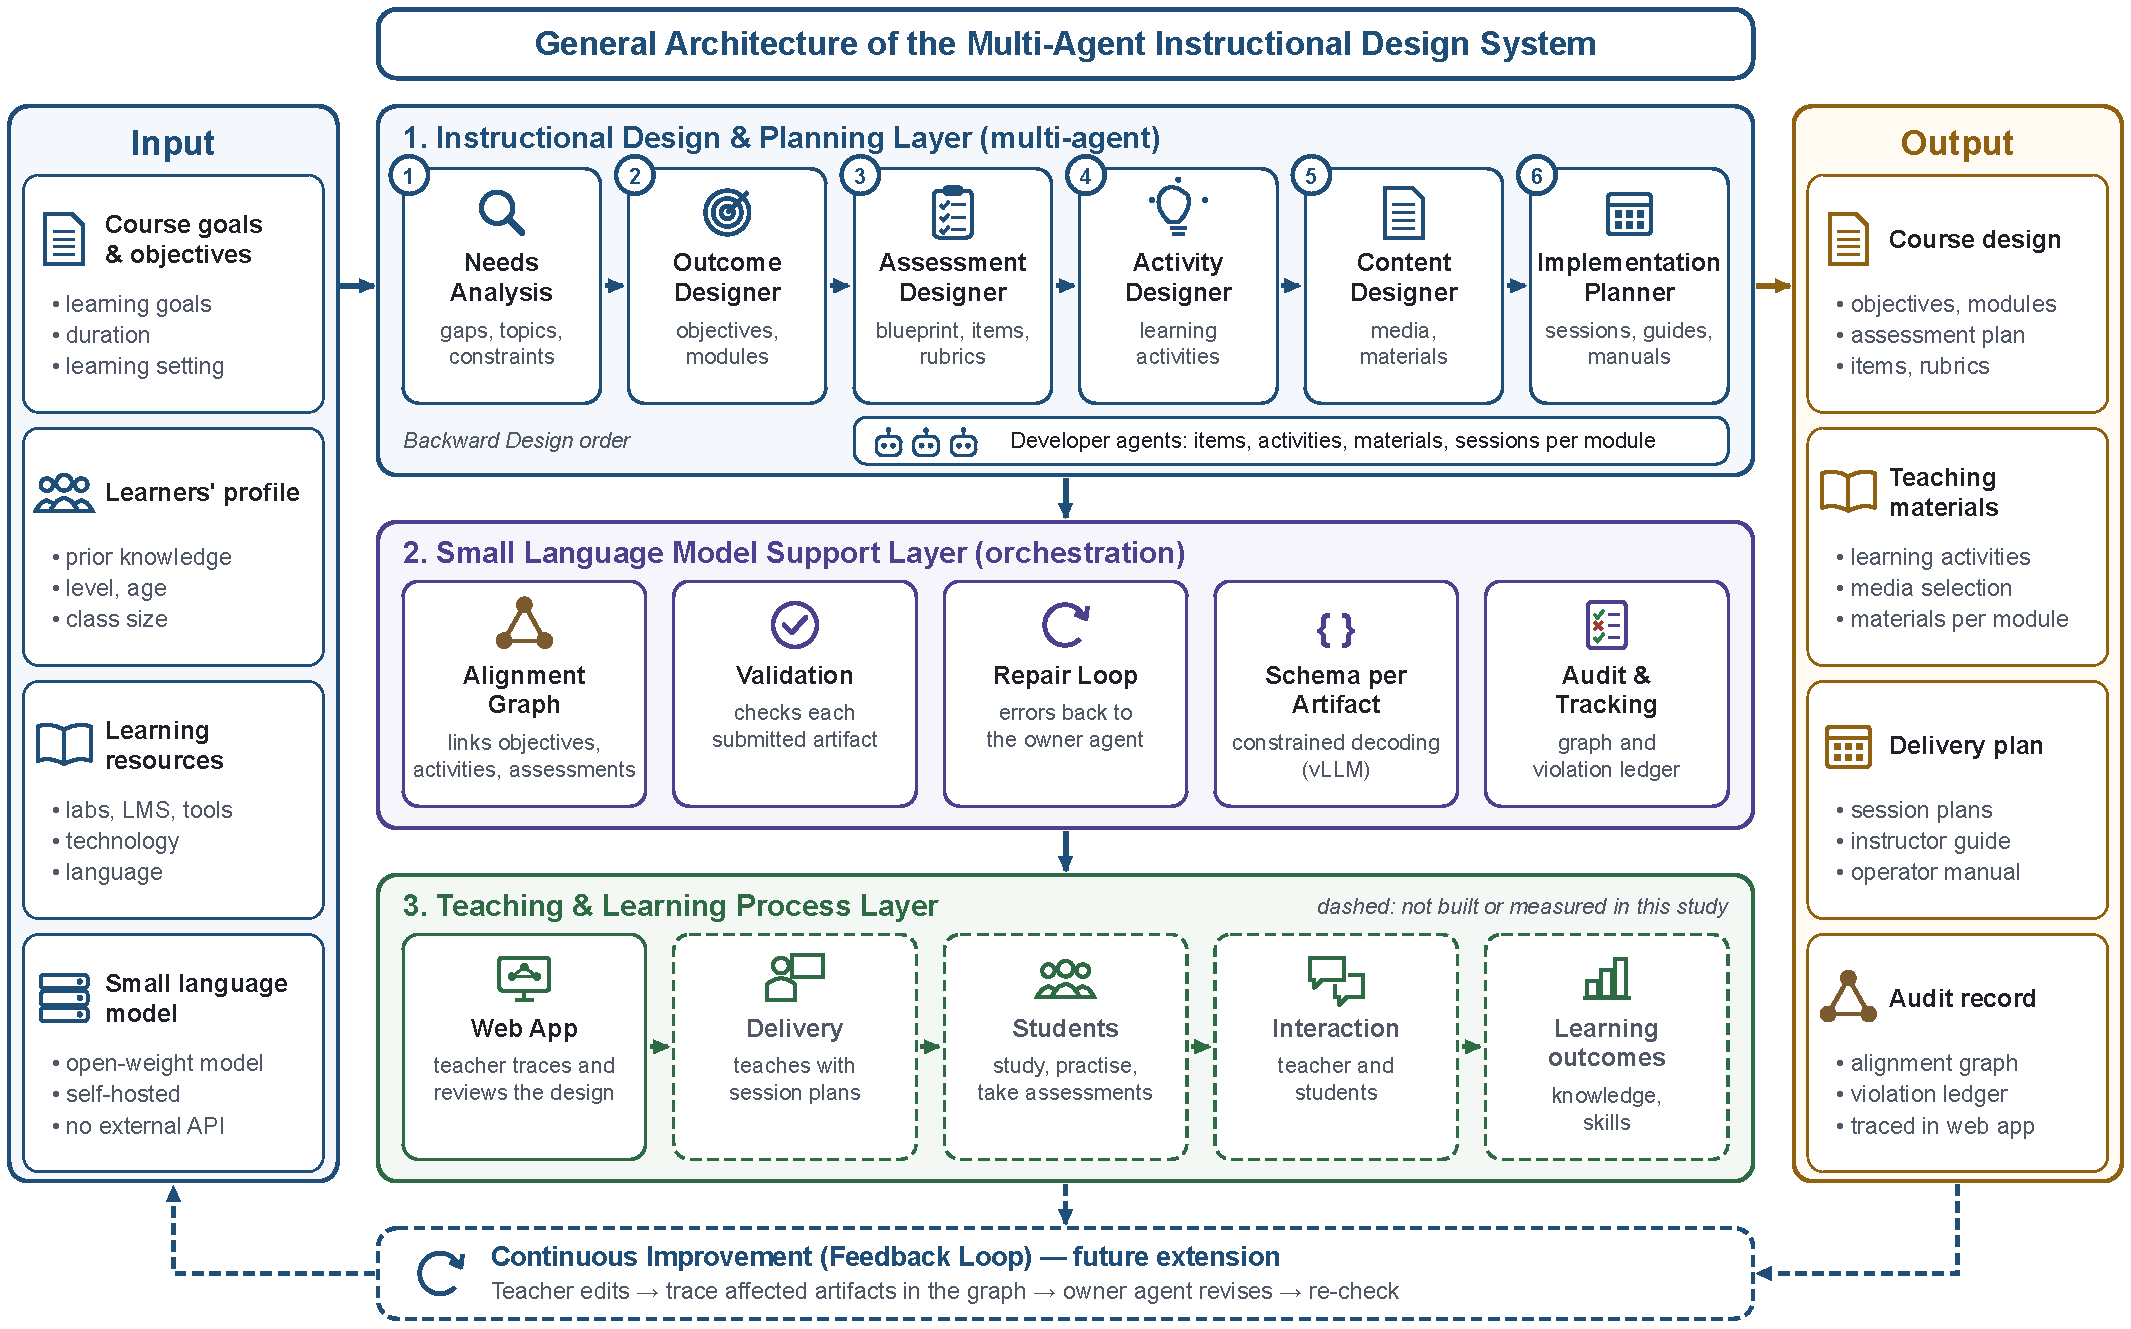
\includegraphics[width=\textwidth]{overview.pdf}
  \caption{Kiến trúc tổng quát của hệ. Lớp 1 gồm sáu tác tử theo công đoạn; lớp 2 là khung
  điều phối quanh SLM; lớp 3 là quá trình dạy và học, nơi giảng viên dùng bản thiết kế. Các khối nét
  đứt ở lớp 3 và vòng cải tiến là bối cảnh sử dụng và hướng mở rộng, không thuộc phạm vi thực
  nghiệm.}
  \label{fig:arch}
\end{figure*}

Hình~\ref{fig:arch} trình bày kiến trúc tổng quát của hệ. Đầu vào là một bản mô tả yêu cầu
thiết kế (design brief): mục tiêu khóa học, hồ sơ người học, bối cảnh và ràng buộc. Hệ gồm ba
lớp. Lớp thiết kế và lập kế hoạch gồm sáu tác tử, mỗi tác tử đảm nhận một công đoạn. Lớp hỗ trợ SLM là khung
điều phối (harness) bao quanh mô hình. Lớp này giữ đồ thị căn chỉnh, kiểm tra từng sản phẩm,
trả lỗi để tác tử sửa và ghi hồ sơ kiểm toán. Lớp dạy và học là nơi giảng viên xem, truy vết và
duyệt bản thiết kế. Mô hình viết nội dung giảng dạy và quyết định cách thực hiện từng công
đoạn. Khung điều phối quyết định thứ tự
công đoạn, định dạng của từng sản phẩm, việc ghi đồ thị và việc kiểm tra.

Đầu ra gồm bản thiết kế khóa học theo cấu trúc ADDIE và hồ sơ kiểm toán. Bản thiết kế có mục
tiêu và mô-đun, kế hoạch đánh giá kèm câu hỏi và rubric, hoạt động, học liệu, kế hoạch buổi học
và tài liệu giảng viên; hồ sơ kiểm toán gồm đồ thị căn chỉnh và sổ vi phạm (violation ledger).

\subsection{Sáu công đoạn}
\label{sec:stages}

\begin{table}[t]
  \caption{Sáu công đoạn, sản phẩm và các kiểm tra chính}
  \label{tab:stages}
  \centering
  \footnotesize
  \setlength{\tabcolsep}{3pt}
  \begin{tabular}{@{}>{\raggedright}p{1.55cm}>{\raggedright}p{2.95cm}>{\raggedright\arraybackslash}p{3.2cm}@{}}
    \toprule
    Công đoạn & Sản phẩm & Kiểm tra chính \\
    \midrule
    1. Phân tích nhu cầu & khoảng trống năng lực, hồ sơ người học, chủ đề, ràng buộc & đủ các trường bắt buộc \\
    2. Mục tiêu, mô-đun & mục tiêu kèm động từ và mức Bloom; mô-đun kèm thời lượng & động từ khớp mức Bloom; mô-đun phủ mục tiêu \\
    3. Đánh giá & bảng đặc tả, nhiệm vụ đánh giá, câu hỏi kèm rubric & mỗi mục tiêu được đánh giá, có câu hỏi ở mức không thấp hơn mục tiêu \\
    4. Hoạt động & hoạt động học tập theo mô-đun & hoạt động luyện mục tiêu và chuẩn bị cho đánh giá; ngân sách thời gian \\
    5. Học liệu & lựa chọn phương tiện, học liệu & học liệu thuộc mô-đun, đúng phương tiện đã chọn \\
    6. Triển khai & kế hoạch buổi học, tài liệu giảng viên, tài liệu vận hành & mọi hoạt động và học liệu được xếp vào buổi học \\
    \bottomrule
  \end{tabular}
\end{table}

Bảng~\ref{tab:stages} liệt kê sáu công đoạn. Thứ tự công đoạn tuân theo Backward Design: xác định kết quả mong muốn trước, sau đó đến bằng chứng đánh giá và cuối
cùng là kế hoạch học tập~\cite{wiggins2005ubd}. Thứ tự này cố định. Tác tử tự chủ trong cách
thực hiện một công đoạn nhưng không chọn công đoạn kế tiếp. Ở bốn công đoạn sau, số sản phẩm
tăng theo quy mô khóa học. Các sản phẩm này do tầng tác tử phát triển (Developer) viết theo
từng mô-đun. Mỗi Developer nhận một nhóm việc được suy ra từ thiết kế đã có. Bộ tổng hợp sắp
xếp nội dung thành năm pha ADDIE theo định dạng mà benchmark yêu cầu.

\subsection{Đồ thị căn chỉnh}
\label{sec:graph}

Trạng thái dùng chung của các tác tử là một đồ thị có hướng
\begin{equation}
\label{eq:graph}
G=(V,E),\qquad E\subseteq V\times V\times\mathcal{R}.
\end{equation}
Mỗi nút $v\in V$ là một sản phẩm thiết kế có kiểu, như mục tiêu, mô-đun, nhiệm vụ đánh giá,
hoạt động hay học liệu. Mỗi cạnh $(u,v,r)$ nối hai sản phẩm qua một kiểu quan hệ
$r\in\mathcal{R}$. Ký hiệu $E_r=\{(u,v)\colon(u,v,r)\in E\}$. Ba quan hệ cốt lõi là ba cạnh
của tam giác constructive alignment: $C_2$ nối mục tiêu với nhiệm vụ đánh giá đo nó, $C_3$ nối mục
tiêu với hoạt động luyện tập nó, và $C_4$ nối hoạt động với nhiệm vụ đánh giá mà nó chuẩn bị.
Các quan hệ còn lại ghi nguồn gốc và cách tổ chức theo mô-đun.

Một mục tiêu $o$ được căn chỉnh về cấu trúc khi tam giác khép kín trên nó:
\begin{equation}
\label{eq:aligned}
\begin{aligned}
\mathrm{aligned}(o)\iff\exists\,h,d\colon\;&(o,h)\in E_{C_3}\wedge(o,d)\in E_{C_2}\\
&\wedge(h,d)\in E_{C_4},
\end{aligned}
\end{equation}
trong đó $h$ là một hoạt động và $d$ là một nhiệm vụ đánh giá. Ba cạnh phải gặp nhau trên
cùng một hoạt động và cùng một nhiệm vụ. Với mỗi quan hệ $r$, gọi $S_r$ là tập nút được xét (mục tiêu với
$C_2$ và $C_3$, nhiệm vụ đánh giá với $C_4$) và $N_r(v)$ là tập nút nối với $v$ qua $r$. Độ phủ của $r$ là
\begin{equation}
\label{eq:coverage}
\mathrm{cov}(r)=\frac{\bigl|\{v\in S_r\colon N_r(v)\neq\emptyset\}\bigr|}{|S_r|}.
\end{equation}
Ví dụ, $\mathrm{cov}(C_2)$ là tỉ lệ mục tiêu có ít nhất một nhiệm vụ đánh giá đo nó. Hai đại
lượng này cho biết quan hệ có tồn tại hay không, không cho biết thiết kế có giá trị sư phạm hay
không. Một cạnh vẫn được tính khi phép kiểm tra mức Bloom gắn cờ nó; cờ này được báo riêng trong
sổ vi phạm.

Mô hình không trực tiếp tạo cạnh. Với ba quan hệ cốt lõi, mỗi sản phẩm khai báo mã định danh (id) của sản phẩm mà nó
phục vụ, ví dụ một hoạt động khai báo mục tiêu mà nó luyện tập. Khi ghi sản phẩm, khung điều
phối tra từng id và tự ghi cạnh có kiểu. Lần nộp mà không id nào trong một trường tham chiếu trỏ tới nút có thật bị
từ chối. Vì vậy, độ phủ đo việc mỗi sản phẩm được gắn tới một đích hợp lệ, không đo sự phù hợp về
nội dung. Mức Bloom của mục tiêu, câu hỏi và hoạt động cũng do tác tử khai báo; các phép kiểm tra so
sánh những nhãn và id này, không đọc lại nội dung văn bản.

\subsection{Kiểm tra, sửa và khả năng mở rộng}
\label{sec:repair}

Mỗi tác tử làm việc theo vòng lặp hành động--quan sát theo kiểu ReAct~\cite{yao2023react}, hiện
thực bằng cơ chế gọi công cụ của mô hình.
Tác tử đọc phần đồ thị thuộc phạm vi vai của mình, rồi nộp sản phẩm qua một công cụ nộp riêng. Khung
điều phối kiểm tra mỗi lần nộp theo định dạng của sản phẩm. Lần nộp hợp lệ được ghi thành nút
kèm các cạnh. Lần nộp không hợp lệ bị từ chối, và thông báo lỗi trở thành quan sát kế tiếp để
tác tử sửa. Sau mỗi công đoạn, các phép kiểm tra trong Bảng~\ref{tab:stages} chạy mà không gọi
mô hình. Khung điều phối tự sửa các vi phạm chỉ cần sắp xếp lại cấu trúc. Các vi phạm cần viết
thêm nội dung được trả lại cho tác tử phụ trách khi tác tử đó còn đang làm việc; vi phạm phát
hiện muộn hơn được ghi vào sổ để giảng viên xem. Khung điều phối không tự viết nội dung giảng
dạy; riêng bản tóm tắt kiểm tra trong đầu ra do khung điều phối tổng hợp từ sổ vi phạm.
Mỗi vi phạm được ghi vào sổ vi phạm cùng kết quả xử lý của nó.

Vì mỗi sản phẩm là một nút có id và mỗi quan hệ là một cạnh có kiểu, kiến trúc cho phép mở rộng
thành vòng cải tiến cục bộ (khối nét đứt ở Hình~\ref{fig:arch}): khi giảng viên sửa một sản phẩm,
hệ lần theo cạnh để tìm các sản phẩm liên quan, giao lại cho đúng tác tử và chỉ kiểm tra lại phần
đó. Vòng cải tiến này chưa được hiện thực trong nghiên cứu này.

\section{THỰC NGHIỆM VÀ ĐÁNH GIÁ}
\label{sec:experiments}

\begin{figure*}[t]
  \centering
  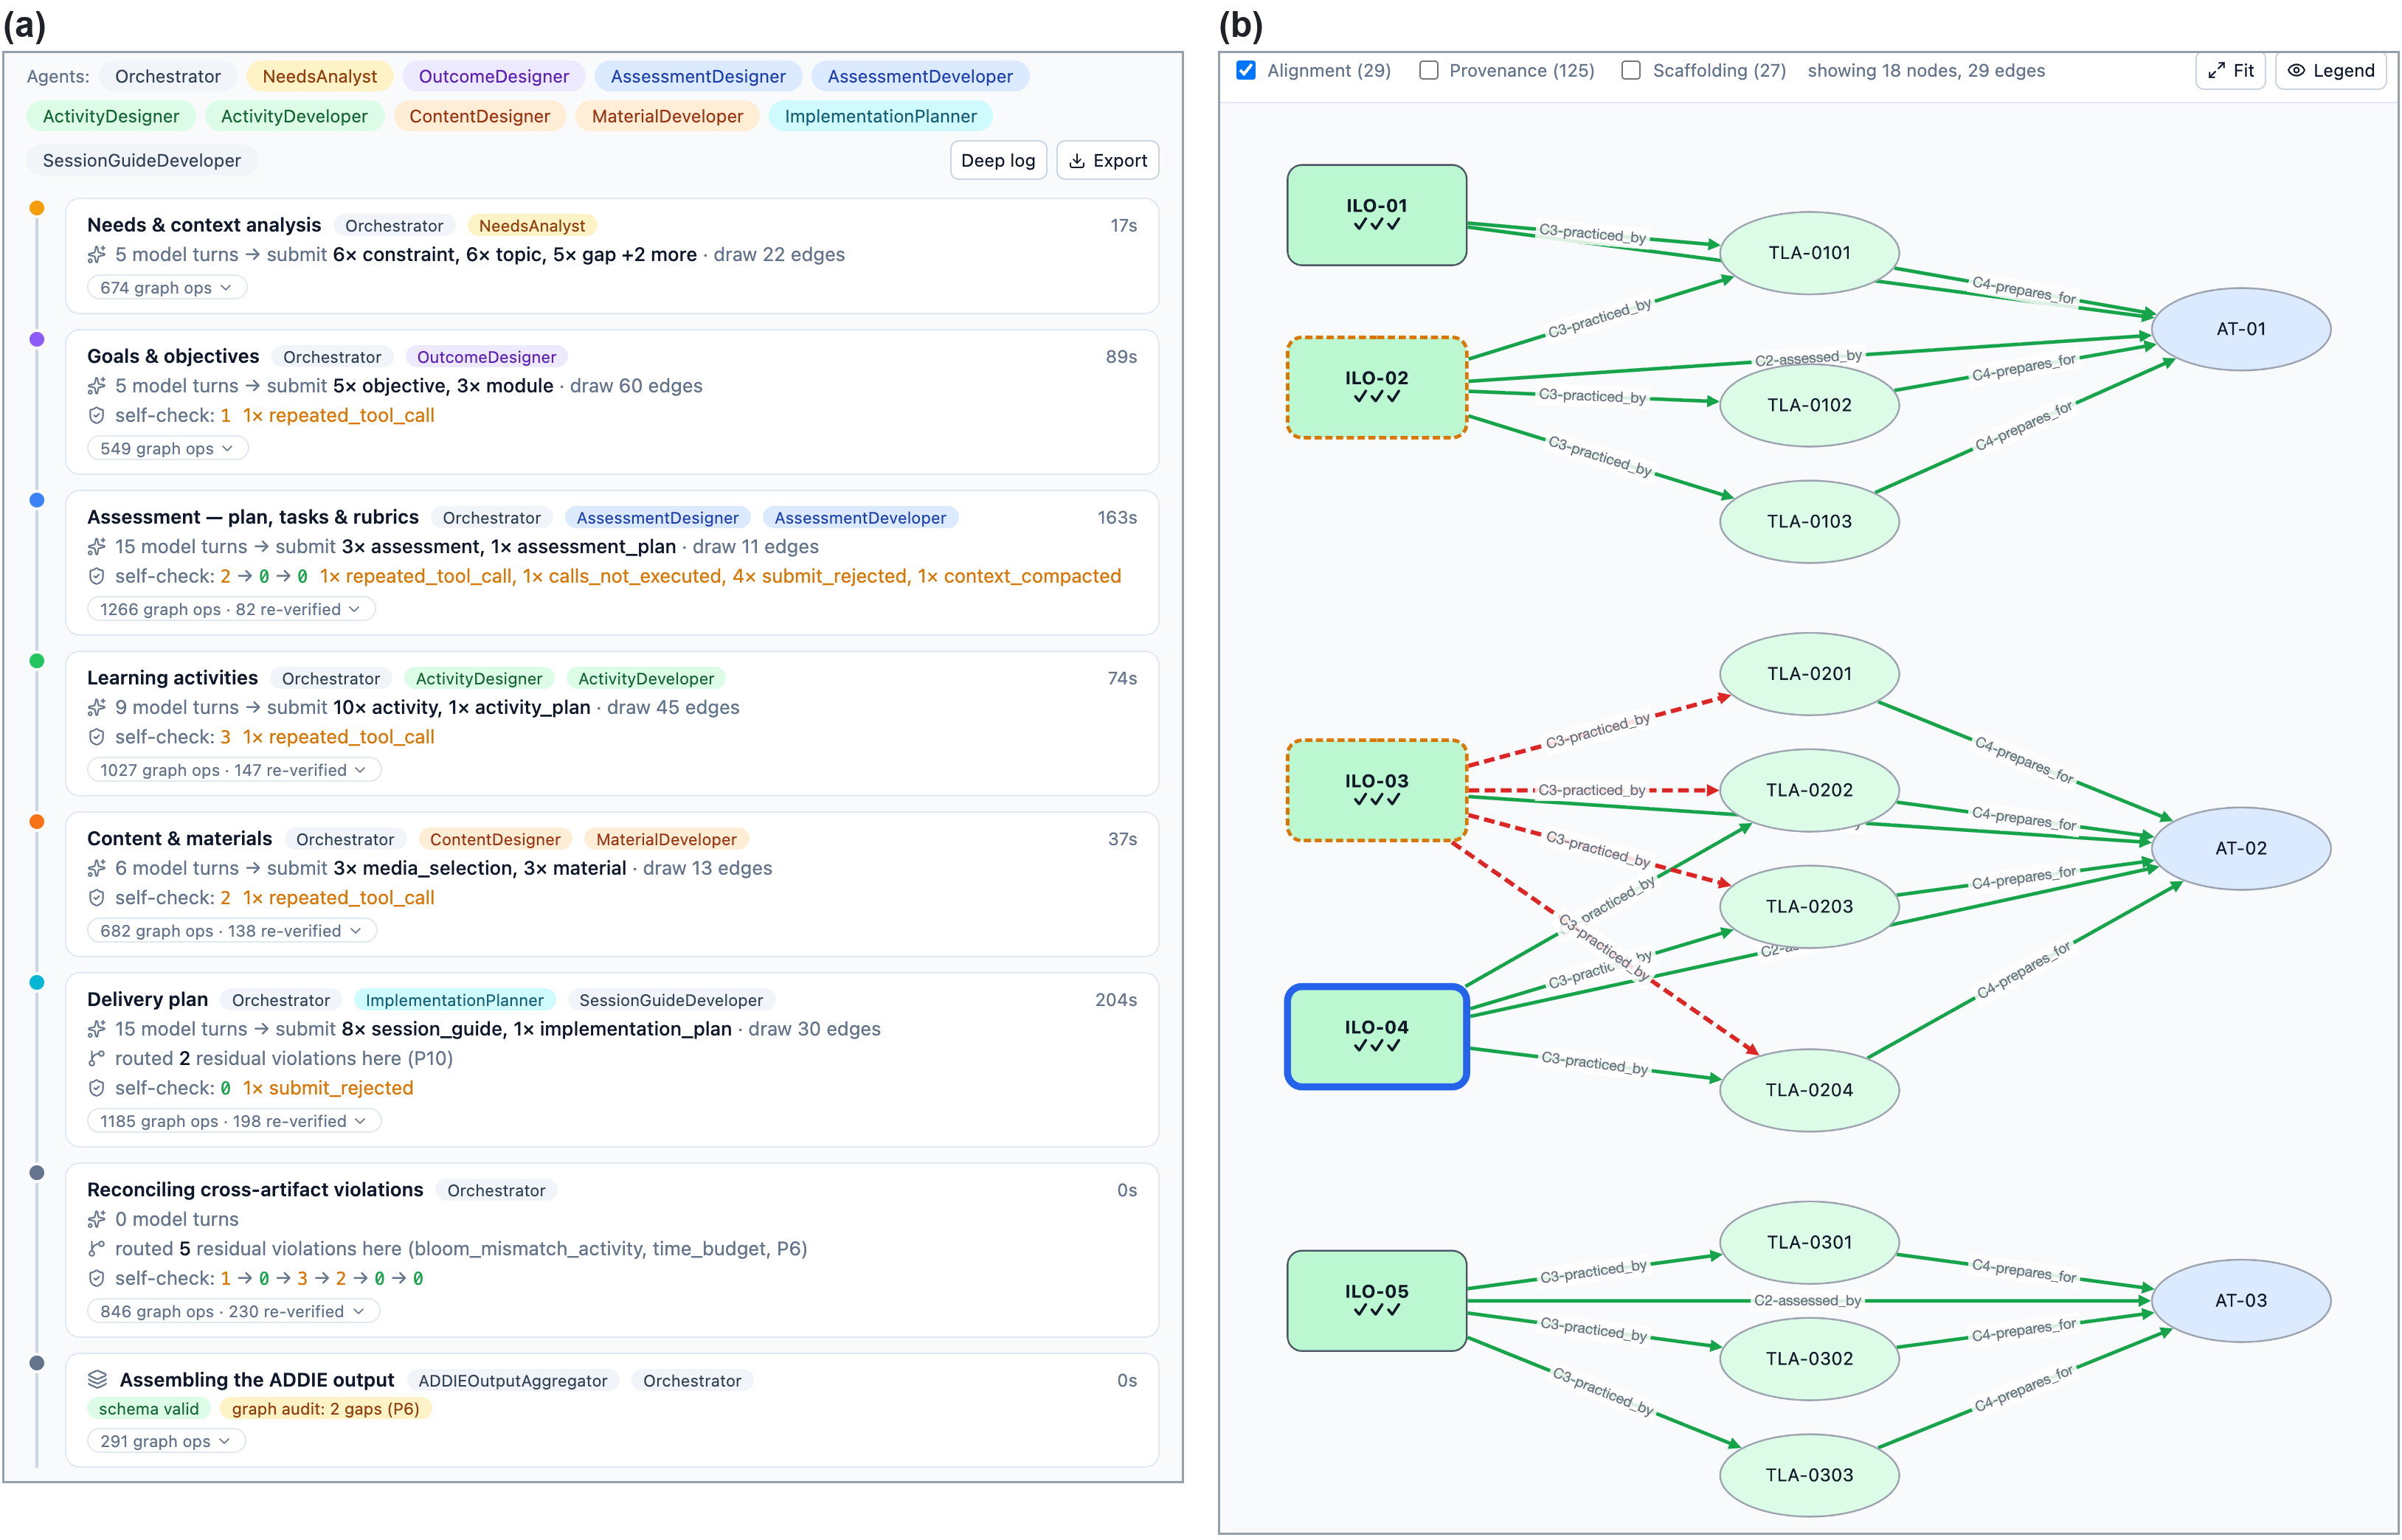
\includegraphics[width=0.86\textwidth]{case.png}
  \caption{Ứng dụng web trên học phần Nhập môn Học máy. (a) Quy trình: sáu công đoạn, bước đối
  chiếu vi phạm và bước tổng hợp, kèm tác tử, sản phẩm đã nộp và kết quả tự kiểm tra.
  (b) Đồ thị căn chỉnh của khóa học ở lớp quan hệ cốt lõi: mục tiêu (ILO), hoạt động (TLA) và
  nhiệm vụ đánh giá (AT); cạnh nét đứt màu đỏ là liên kết không khớp mức Bloom; viền nét đứt màu cam đánh dấu mục tiêu có phép
  kiểm tra không đạt.}
  \label{fig:case}
\end{figure*}

\subsection{Thiết lập thực nghiệm}
\label{sec:setup}

Chúng tôi dùng kịch bản, sáu tác tử đối chứng, rubric và bộ chấm của
ISD-Agent-Bench~\cite{isdagentbench}; bộ chạy thực nghiệm do chúng tôi viết. Tập đánh giá gồm
\NScen{} kịch bản thuộc tập kiểm tra, tách biệt với 10 kịch bản đã dùng khi hoàn thiện hệ. Các kịch bản viết bằng tiếng Anh. Hệ đề xuất được so sánh với sáu tác tử
của benchmark: EduPlanner (bản hiện thực lại trong benchmark, dựa trên~\cite{zhang2025eduplanner}),
Baseline (sinh một lượt), React-ADDIE (còn gọi là ReAct-ISD, kết hợp ADDIE với
ReAct~\cite{yao2023react}), ADDIE-Agent, Dick-Carey-Agent và RPISD-Agent. Tên tác tử theo bài báo gốc; prompt của
React-ADDIE được dịch sang tiếng Anh, không đổi phương pháp. Mọi hệ chạy trên cùng mô hình
Qwen3.5-2B, phục vụ bằng vLLM~\cite{kwon2023vllm} trên máy chủ GPU tự triển khai, với nhiệt độ
sinh mặc định 0.7 (EduPlanner giữ nhiệt độ riêng cho từng vai theo thiết kế gốc) và trần 8192
token cho mỗi lượt gọi, ứng với ngân sách của một GPU đơn 12--16\,GB mà nghiên cứu hướng tới.
Chế độ suy luận (thinking) được bật nhưng giới hạn ở 32 token trong cùng trần đó, như nhau cho
mọi hệ, và được cố định trước khi chạy chính thức. Mỗi cặp (hệ, kịch bản) được sinh đầu ra một lần; vì nhiệt độ
khác không, kết quả của một lần sinh không tất định. Khi một lần nộp bị từ chối, hệ đề xuất viết lại sản phẩm đó
một lần bằng giải mã có ràng buộc theo JSON Schema, một cơ chế sẵn có của vLLM dựa trên các backend như
XGrammar~\cite{vllmstructured,dong2025xgrammar}; các tác tử đối chứng giữ nguyên phương pháp
và không có bước này.

Ba LLM judge (mô hình LLM dùng để chấm điểm) thuộc ba họ mô hình khác nhau (GPT-6 Luna,
Gemini~3.1 Flash-Lite, DeepSeek-V4.1-Flash) chấm mỗi đầu ra ở chế độ tắt suy luận; điểm cuối
cùng là trung vị của ba điểm, để một LLM judge lệch không chi phối kết quả. Không họ nào
trùng với họ của mô hình tác tử (Qwen). GPT-6 Luna không nhận tham số nhiệt độ nên không tất định. Điểm ADDIE (0--100) đánh giá sản phẩm
theo 33 tiêu chí con. Điểm Trajectory đánh giá quá trình gọi công cụ; theo mã nguồn bộ chấm của benchmark, LLM judge
chỉ nhận 20 lời gọi công cụ đầu tiên~\cite{isdagentbench}, nên hệ có nhiều lời gọi, như hệ đề xuất, chịu bất lợi ở điểm này. Điểm
Total bằng
$0.7\cdot\mathrm{ADDIE}+0.3\cdot\mathrm{Trajectory}$. Hệ đề xuất được so sánh với từng hệ còn
lại bằng kiểm định Wilcoxon theo cặp kịch bản, hiệu chỉnh Holm trong từng điểm. Một hệ không tạo
ra đầu ra chấm được ở kịch bản nào thì nhận 0 điểm ở kịch bản đó.

\subsection{Kết quả trên benchmark}
\label{sec:results}

\begin{figure*}[t]
  \centering
  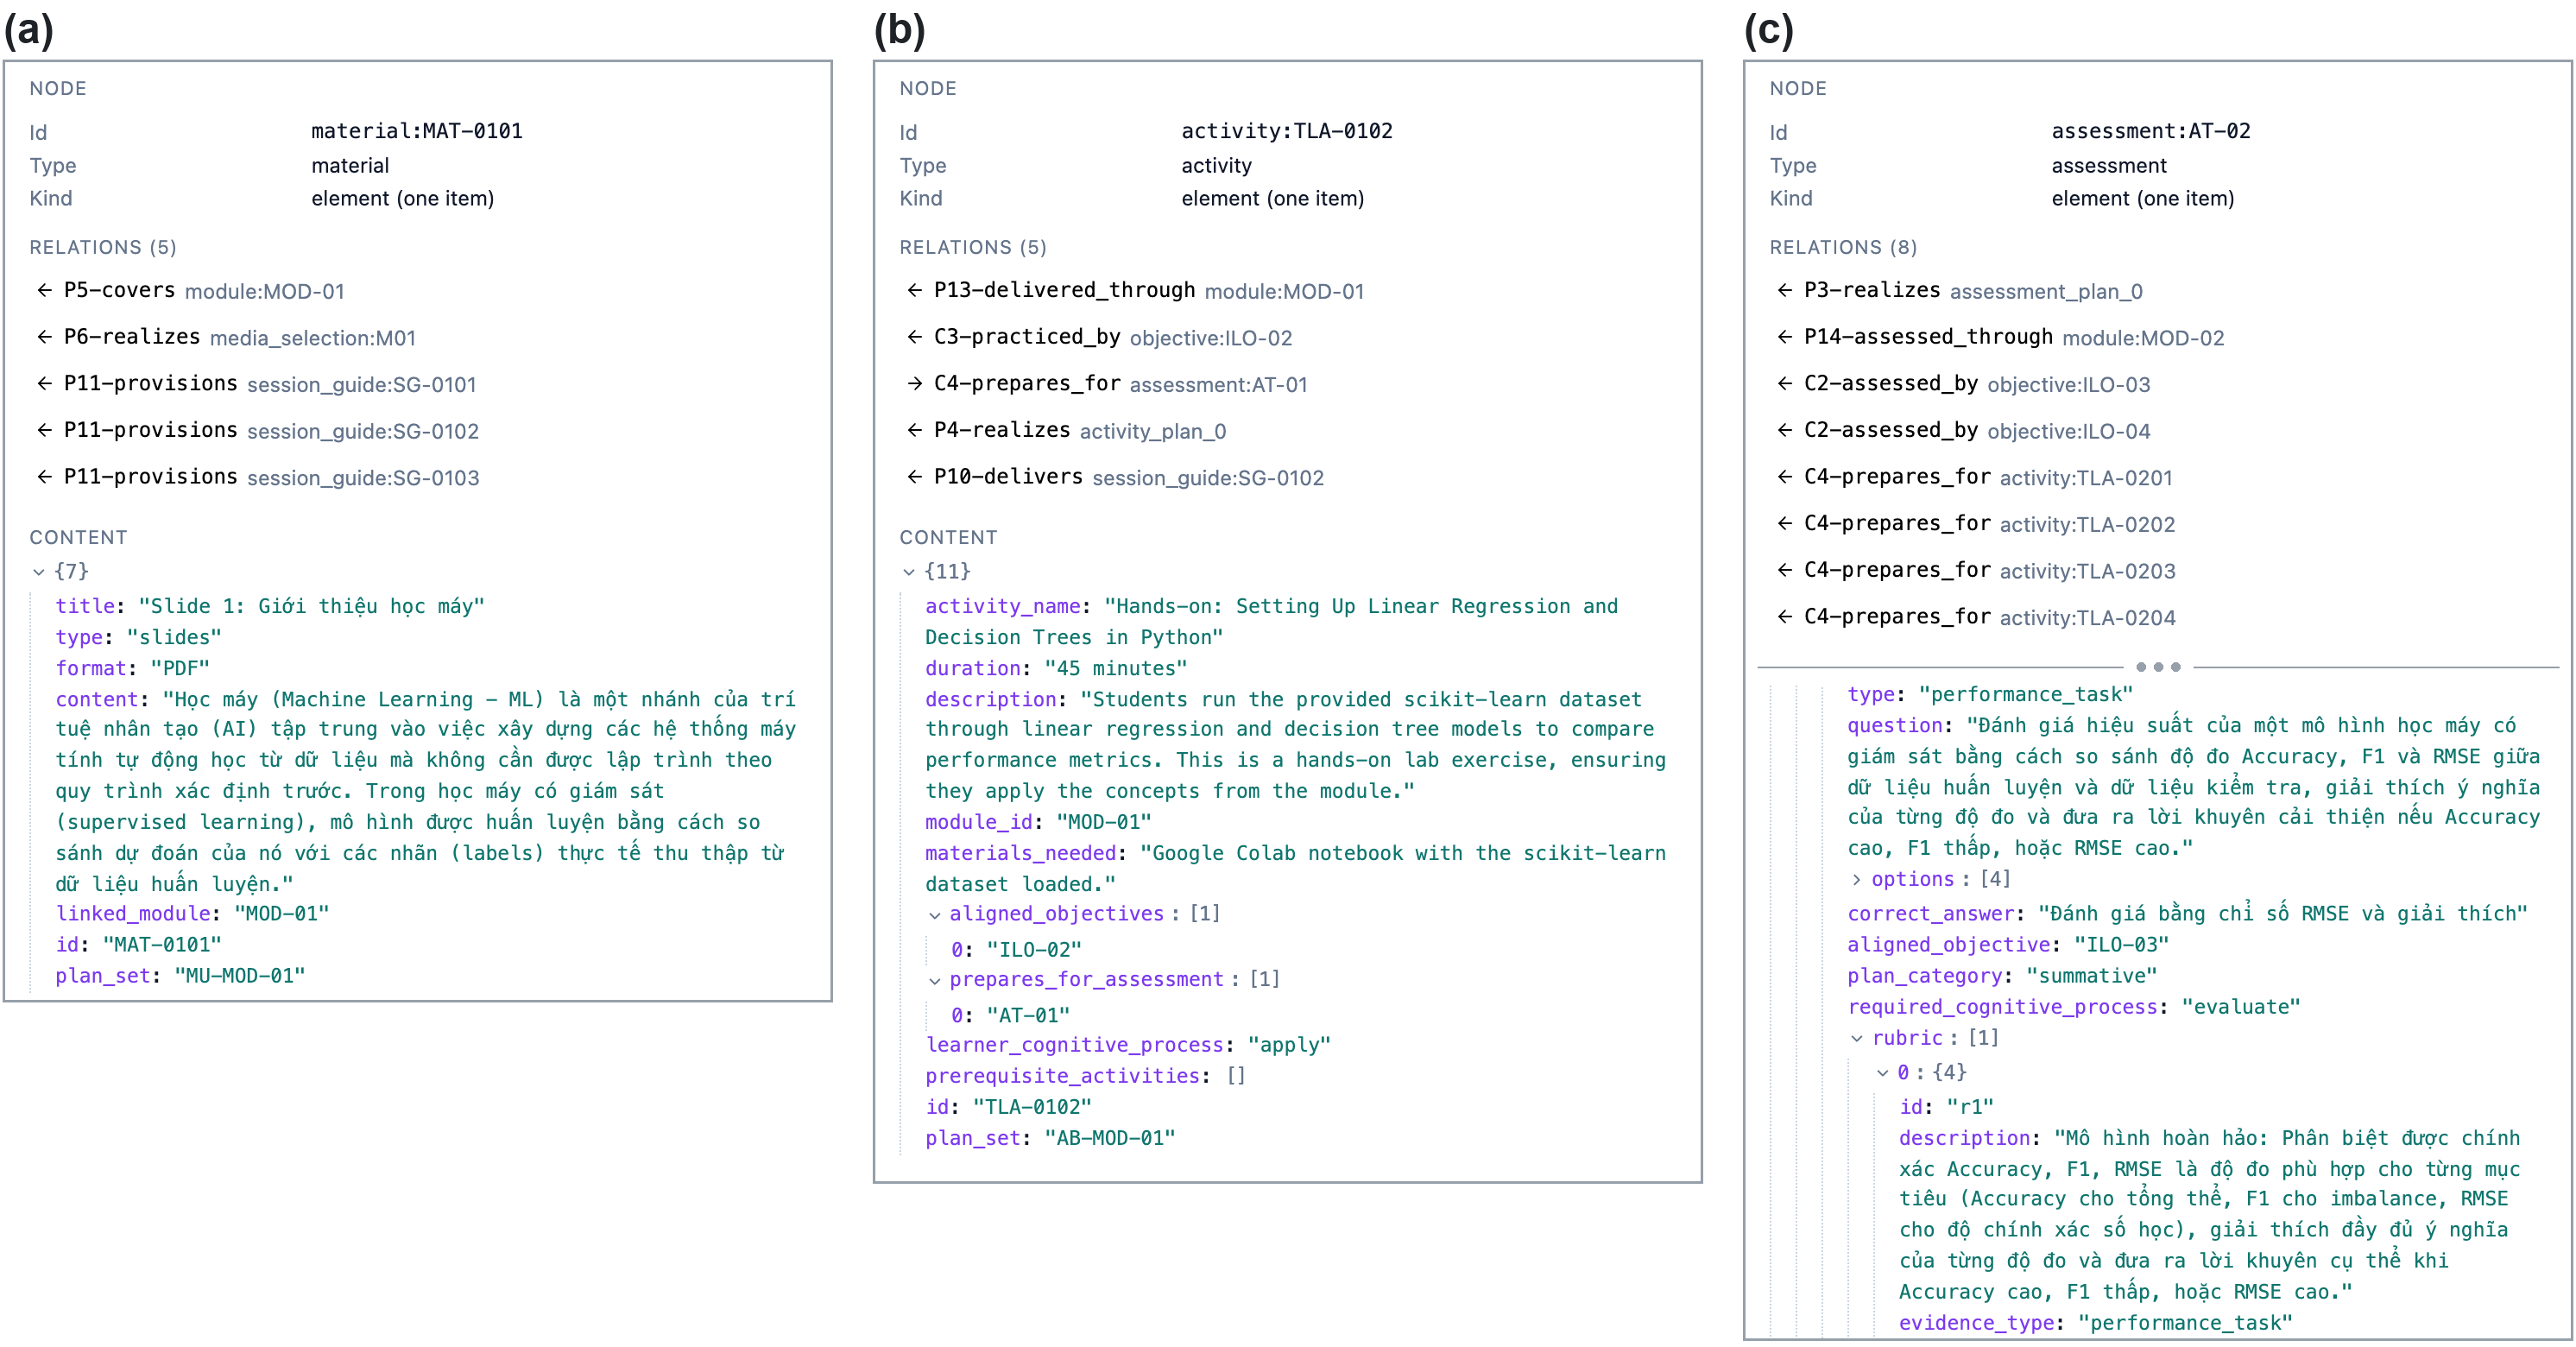
\includegraphics[width=0.88\textwidth]{case_outputs.png}
  \caption{Ba sản phẩm đầu ra trên giao diện, mỗi sản phẩm kèm các quan hệ của nó trong đồ thị.
  (a) Học liệu MAT-0101 (slide), thuộc mô-đun MOD-01 và được dùng ở \caseMatSessions{} buổi học. (b) Hoạt động
  TLA-0102, luyện mục tiêu ILO-02 và chuẩn bị cho nhiệm vụ đánh giá AT-01. (c) Nhiệm vụ đánh giá
  tổng kết AT-02, đo \caseTaskObjs{} mục tiêu và được \caseTaskActs{} hoạt động chuẩn bị, cùng một câu hỏi của nó kèm
  tiêu chí rubric; dải chấm đánh dấu phần nội dung được lược bớt. Các quan hệ P ghi nguồn gốc và
  cách tổ chức theo mô-đun.}
  \label{fig:outputs}
\end{figure*}

\begin{figure*}[t]
  \centering
  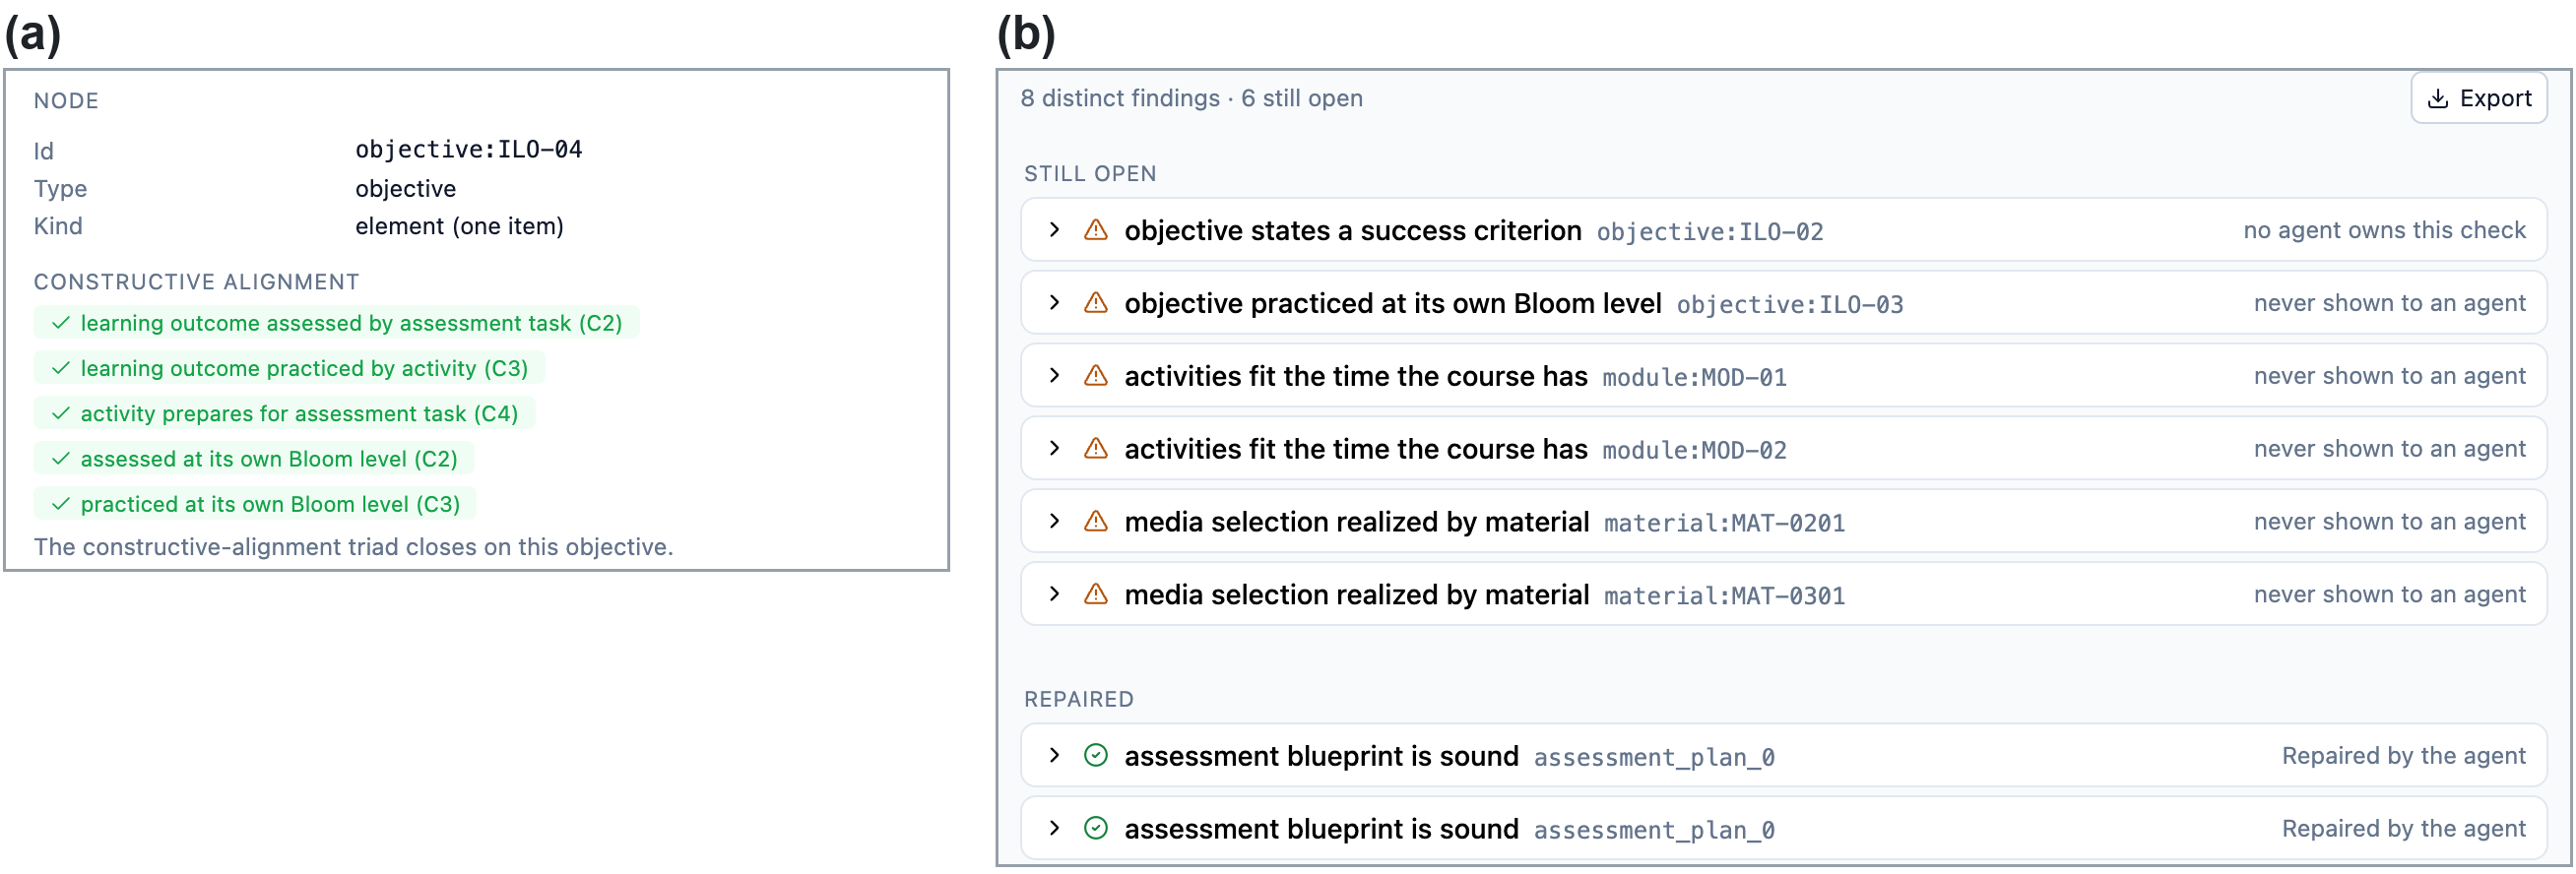
\includegraphics[width=0.88\textwidth]{case_audit.png}
  \caption{Hồ sơ kiểm toán trên giao diện. (a) Mục tiêu ILO-04 khép kín tam giác $C_2$--$C_4$ và các phép kiểm tra mức Bloom của nó.
  (b) Sổ vi phạm: các vi phạm còn mở và các vi phạm đã được sửa, kèm bên đã sửa.}
  \label{fig:audit}
\end{figure*}

\begin{table}[t]
  \caption{Điểm của mô hình chấm trên ISD-Agent-Bench (trung bình $\pm$ độ lệch chuẩn qua 30 kịch bản) và token mỗi kịch bản}
  \label{tab:judge}
  \centering
  \footnotesize
  \setlength{\tabcolsep}{2.5pt}
  \begin{tabular}{@{}lcccc@{}}
    \toprule
    Hệ & ADDIE $\uparrow$ & Trajectory $\uparrow$ & Total $\uparrow$ & Token (k) $\downarrow$ \\
    \midrule
    Hệ thống đề xuất & 59.0\,$\pm$\,2.8 & 69.7\,$\pm$\,5.9 & 62.2\,$\pm$\,2.3 & 282 \\
    EduPlanner & 30.0\,$\pm$\,19.8$^{*}$ & 53.0\,$\pm$\,32.7 & 36.9\,$\pm$\,23.2$^{*}$ & 70 \\
    Baseline & 43.4\,$\pm$\,17.7$^{*}$ & 69.2\,$\pm$\,19.0 & 51.1\,$\pm$\,16.6$^{*}$ & 10 \\
    React-ADDIE & \textbf{59.1\,$\pm$\,6.7} & 71.5\,$\pm$\,9.5 & \textbf{62.8\,$\pm$\,4.9} & 15 \\
    ADDIE-Agent & 48.5\,$\pm$\,3.6$^{*}$ & \textbf{81.5\,$\pm$\,3.0$^{*}$} & 58.4\,$\pm$\,2.7$^{*}$ & 23 \\
    Dick-Carey-Agent & 58.0\,$\pm$\,3.0 & 72.6\,$\pm$\,5.6 & 62.4\,$\pm$\,3.1 & 26 \\
    RPISD-Agent & 58.4\,$\pm$\,2.5 & 69.9\,$\pm$\,3.3 & 61.8\,$\pm$\,1.9 & 61 \\
    \bottomrule
  \end{tabular}
  \par\vspace{2pt}
  {\scriptsize\raggedright $^{*}$ khác có ý nghĩa so với hệ thống đề xuất (Wilcoxon theo cặp, Holm trong từng điểm, $p<0.05$).\\ Số kịch bản có dữ liệu token: EduPlanner 22, Baseline 28.\\ Kịch bản không có đầu ra chấm được, tính 0 điểm: EduPlanner 8, Baseline 2.\par}
\end{table}


Bảng~\ref{tab:judge} trình bày điểm LLM judge. Về điểm ADDIE, hệ đề xuất (\cmpAGAddie) không
khác biệt có ý nghĩa với React-ADDIE (\cmpReactAddie; chênh lệch \cmpReactAddieDiff{} điểm, KTC
95\% [\cmpReactAddieCILo; \cmpReactAddieCIHi], $p$\,\cmpReactAddieP), Dick-Carey-Agent
(\cmpDickAddie) và RPISD-Agent (\cmpRpisdAddie). Không khác biệt có ý nghĩa không đồng nghĩa với
tương đương: khoảng cách giữa các hệ này nhỏ hơn nhiều so với độ lệch giữa các LLM judge trên
cùng một đầu ra (\JudgeSD{} điểm). Hệ đề xuất cao hơn ADDIE-Agent
\cmpAddieAddieDiff{} điểm, Baseline \cmpBaseAddieDiff{} điểm và EduPlanner \cmpEduAddieDiff{}
điểm ($p$\,\cmpMaxPAddieBetter{} ở cả ba so sánh). Một phần chênh lệch với Baseline và EduPlanner
đến từ các kịch bản không có đầu ra chấm được: Baseline thất bại vì đầu ra chạm trần 8192
token, còn EduPlanner thất bại vì đầu ra không khớp lược đồ do chính nó quy định. Về điểm
Trajectory, ADDIE-Agent đạt cao nhất (\cmpAddieTraj) và cao hơn có ý nghĩa so với hệ đề xuất
($p$\,\cmpAddieTrajP). Về điểm Total, hệ đề xuất không khác biệt có ý nghĩa với React-ADDIE,
Dick-Carey-Agent và RPISD-Agent. Hệ dùng trung bình \cmpAGTok{}k token
và \cmpAGCalls{} lời gọi mô hình mỗi kịch bản, so với \cmpReactTok{}k token và
\cmpReactCalls{} lời gọi của React-ADDIE, gấp khoảng \cmpTokRatioReact{} lần về số token; thời
gian chạy trung bình là \cmpAGMin{} so với \cmpReactMin{} phút mỗi kịch bản, đo trên máy chủ dùng
chung nên gồm cả thời gian chờ. Hệ có
chi phí tính toán cao hơn đáng kể so với các hệ dạng quy trình gọn nhẹ. Chúng tôi báo cáo chi phí này bên cạnh khả năng truy vết
và kiểm toán, mà không diễn giải rằng hệ hiệu quả hơn về mặt tính toán.

\subsection{Triển khai ứng dụng}
\label{sec:case}

Hệ được đóng gói thành một ứng dụng web. Giảng viên nhập bản mô tả yêu cầu thiết kế, hoặc mô tả
học phần bằng hội thoại, rồi khởi chạy hệ trên một SLM tự triển khai. Trong lúc hệ chạy, quy trình và
đồ thị căn chỉnh được cập nhật dần trên màn hình. Sau khi chạy xong, giảng viên chọn từng nút
để xem nội dung sản phẩm, các quan hệ của nó và các vi phạm còn mở.

Để minh họa, chúng tôi soạn bản mô tả yêu cầu cho học phần Nhập môn Học máy dành cho sinh viên Công nghệ
Thông tin năm thứ ba: 4 tuần (30 giờ), học kết hợp, khoảng 40 sinh viên, thực hành Python
trên Google Colab. Bản mô tả có bốn mục tiêu khóa học: quy trình học có giám sát, cài đặt hồi
quy tuyến tính và cây quyết định, đánh giá mô hình, và xử lý quá khớp. Ngôn ngữ đầu ra yêu cầu
là tiếng Việt. Hệ chạy trên Qwen3.5-2B với cùng cấu hình như Mục~\ref{sec:setup} và hoàn thành
sau khoảng \caseMin{} phút.

Hình~\ref{fig:case}a cho thấy quy trình thực hiện. Hệ sinh \caseObj{} mục tiêu, \caseMod{}
mô-đun, \caseTask{} nhiệm vụ đánh giá với \caseItem{} câu hỏi, \caseAct{} hoạt động,
\caseMat{} học liệu và \caseSess{} kế hoạch buổi học, dùng \caseTok{}k token qua \caseCalls{}
lời gọi mô hình. Trên đồ thị (Hình~\ref{fig:case}b), độ phủ của $C_2$, $C_3$ và $C_4$ là
\caseCovTwo\%, \caseCovThree\% và \caseCovFour\%, và \caseClosed{} trên \caseObj{} mục tiêu
khép kín tam giác (Hình~\ref{fig:audit}a).

Hình~\ref{fig:outputs} trình bày ba loại sản phẩm đầu ra. Học liệu MAT-0101 là slide giới thiệu
học máy, viết bằng tiếng Việt. Hoạt động TLA-0102 là bài thực hành cài đặt hồi quy tuyến tính
và cây quyết định trên Google Colab, kéo dài \caseActMinutes{} phút. Câu hỏi tổng kết của AT-02 yêu cầu so sánh
các độ đo giữa dữ liệu huấn luyện và dữ liệu kiểm tra, gắn với mục tiêu ILO-03 ở mức
\emph{evaluate} và có rubric mô tả từng mức đạt.

Sổ vi phạm (Hình~\ref{fig:audit}b) ghi \caseViol{} vi phạm: \caseViolAgent{} đã được tác tử
sửa, \caseViolOpen{} còn mở. Các vi phạm còn mở chưa được đưa tới tác tử nào, vì được phát hiện
sau khi tác tử phụ trách đã kết thúc hoặc thuộc phép kiểm tra chưa có tác tử phụ trách. Chúng chỉ
cho giảng viên những chỗ cần xem lại: ILO-02 chưa nêu tiêu chí đạt, hoạt động của ILO-03 thấp hơn
mức Bloom của mục tiêu (cạnh nét đứt màu đỏ ở Hình~\ref{fig:case}b), tổng thời lượng hoạt động của
\caseOverrunMods{} mô-đun vượt thời lượng của mô-đun, và \caseMediaMismatch{} học liệu khai loại mô
phỏng nhưng thực chất là kịch bản video. Bản thiết kế còn những lỗi nằm ngoài
phạm vi của các phép kiểm tra. \caseDiagOnlyIds{} chỉ được đo bởi một nhiệm vụ chẩn đoán có trọng
số \caseDiagWeight\%, nên tam giác khép kín về cấu trúc nhưng chưa có đánh giá tổng kết. Mô-đun
thứ hai có các kế hoạch buổi học chồng lấn nhau, và trường mục tiêu của kế hoạch buổi học trỏ tới id
không tồn tại mà không bị phát hiện, vì không quan hệ nào đọc trường đó. Mục tiêu, câu hỏi, rubric và học liệu được viết bằng
tiếng Việt, nhưng kế hoạch đánh giá, các sản phẩm của pha triển khai và các hoạt động của mô-đun
đầu tiên được viết bằng tiếng Anh (Hình~\ref{fig:outputs}b); một phần do khung điều phối sinh từ
mẫu cố định. Một mục tiêu gọi kiểm chứng chéo là kỹ thuật điều chuẩn. Các lỗi
này cho thấy bản thiết kế do SLM sinh ra vẫn cần giảng viên rà soát trước khi dùng.

\subsection{Thảo luận}
\label{sec:discussion}

\textbf{(1) Đầu ra truy vết được.} Mỗi quan hệ mục tiêu--hoạt động--đánh giá là một cạnh có thể
xem trên giao diện. Giao diện cho phép giảng viên xem mục tiêu nào chưa được đánh giá hay chưa có hoạt động
luyện tập, thay vì phải đọc lại toàn bộ bản thiết kế. Các phép kiểm tra chỉ là kiểm tra cấu trúc,
không phát hiện lỗi chuyên môn hay lỗi ngôn ngữ.

\textbf{(2) Nền tảng cho cải tiến cục bộ.} Với vi phạm còn mở của \caseLocalObjective, đồ thị
chỉ ra \caseLocalRewrite{} hoạt động là ứng viên cần viết lại và \caseLocalCheck{} sản phẩm liền kề
cần rà soát cùng: nhiệm vụ đánh giá, mô-đun, mục tiêu và kế hoạch buổi học liên quan;
\caseLocalOutside{} trên \caseDesign{} sản phẩm thiết kế nằm ngoài lân cận một cạnh này. Đây là
phạm vi đọc trực tiếp từ đồ thị, chưa phải phân tích lan truyền; việc hiện thực vòng sinh lại cục
bộ là hướng phát triển của nghiên cứu.

\textbf{Hạn chế.} Thực nghiệm chỉ dùng một mô hình (Qwen3.5-2B), \NScen{} kịch bản và một lần sinh cho mỗi
cặp. LLM judge có những thiên lệch đã được ghi nhận~\cite{ye2025justice}; độ lệch chuẩn giữa ba LLM judge trên
cùng một đầu ra trung bình \JudgeSD{} điểm ADDIE. Ba LLM judge này thay cho cặp LLM judge mặc
định trong mã nguồn của benchmark (GPT-4o-mini và Gemini 2.5 Flash-Lite), và thứ hạng giữa hệ đề xuất và
React-ADDIE thay đổi theo từng LLM judge. Hệ đề xuất được hoàn thiện trên chính mô hình này và có
thêm bước giải mã có ràng buộc, trong khi các tác tử đối chứng chạy nguyên phương pháp; phép so sánh
vì vậy đánh giá cả gói hệ thống, không tách riêng đóng góp của kiến trúc. Trường hợp minh họa là một học phần, một lần chạy, chưa được đưa vào giảng dạy và chưa có
đánh giá của chuyên gia hay của người học. Với đầu ra tiếng Việt, SLM 2B còn trộn ngôn ngữ và
mắc lỗi chuyên môn, và các mẫu văn bản của khung điều phối chưa được bản địa hóa.

\section{KẾT LUẬN VÀ HƯỚNG PHÁT TRIỂN}
\label{sec:conclusion}

Bài báo đã trình bày một hệ đa tác tử thiết kế giảng dạy chạy trên SLM tự triển khai. Hệ chia
quy trình thành sáu công đoạn, các tác tử dùng chung một đồ thị căn chỉnh, và đầu ra kèm hồ sơ
kiểm toán. Trên \NScen{} kịch bản với Qwen3.5-2B, điểm ADDIE của hệ không khác biệt có ý nghĩa
với tác tử mạnh nhất của benchmark, với chi phí token cao hơn khoảng \cmpTokRatioReact{} lần. Hệ
được đóng gói thành ứng dụng web và được dùng để thiết kế một học phần Công nghệ Thông tin với
đầu ra tiếng Việt. Hướng phát triển gồm vòng chỉnh sửa có giảng viên
tham gia và sinh lại cục bộ theo đồ thị, đánh giá trên nhiều cỡ mô hình, và lấy nhận xét của
chuyên gia thiết kế giảng dạy trên các học phần thực tế.

\bibliographystyle{IEEEtran}
\bibliography{refs}

\end{document}
